\lecture{25}{2025-05-20}{Still linear codes}{}


\begin{parag}{Minimum distance over the parity check matrix}
	\begin{theoreme}
	     Let $H$ be any parity check matrix of a linear code. The minimum distance of the code is the smallest positive integer $d$ such that there are $d$ columns of $H$ that are linearly dependent.
	\end{theoreme}
	\begin{subparag}{In other words}
	    This means that, if you take $d_{min}$, then there exists some column that are linearly dependent. (I think this was on the exercise set of last week)
	\end{subparag}
	\begin{subparag}{Proof}
	    For a linear code, the minim distance is the smallest weight of a non zero vector codeword. Let $\vec{c} \neq \vec{0}$ be a codeword with the smallest weight $d_{min}$. The fact that $\vec{c}H^T =  \vec{0}$ proves that $H$ has $d_{min}$ linearly dependent columns.\\
	    We need to argue that fewer than $d$ columns of $H$ are not linearly dependent. Suppose that $H$ has $t < d$ linearly dependent columns. Then we could find a non zero codeword $\vec{c}$ of weight smaller than $d$ such that $\vec{c}H^T =  0$ which is a contradiction.

	\end{subparag}
    
	\begin{framedremark}
	  for the first fact, $\vec{c}H^T =  0$ proves that $H$ has $d$ linearly dependent columns. You can see it first like this. If you take a vector with a weight of $d$ then you know that if you take the multiplication like this: $\vec{c}H^T$ you multiply every columns of $H$ by an element of $\vec{c}$ (like each column of $H^T$ is multiplied by a scalar (not a litteraly scalar in $\mathbb{R}$)) therefore you have like imagine you vector lie this:
	  \begin{align*} 
		  \vec{c} =  \begin{pmatrix} 1 \\ 0 \\ 2 \end{pmatrix} 
	  \end{align*}
	  Then if you take the multiplication said before you get something like this:
	  \begin{align*} 
		  c_1 \star  \text{col}_1 + \overbrace{c_2}^{= 0} \star  \text{col}_2 + c_3 \star  \text{col}_3 =  0
	  \end{align*}
	  But because we know the weight is $d$ (here 2) then you know that  there is $d$ column such that a non-trivial equation gives $0$, therefore, there are linearly dependent.
	\end{framedremark}
\end{parag}





\begin{parag}{Example}
    The following is a parity check matrix for a Hamming code of parameters $n =  7$, $k =  4$.
    \begin{align*} 
	    H =  \begin{pmatrix} 1 & 0 & 1 & 0 & 1 & 0 & 1 \\ 0 & 1 & 1 & 0 & 0 & 1 & 1 \\ 0 & 0 & 0 & 1 & 1 & 1 & 1 \end{pmatrix} 
    \end{align*}
    Clearly no two columns are linearly dependent. Column, 1, 2 and $3$ are linearly dependent.\\
    Hence $d_{min} =  3$.
\end{parag}

\subsubsection{Standard Array: Background Material}

\begin{parag}{Equivalence Relation (review)}
    \begin{itemize}
	    \item $\mathcal{G}$ a set
	    \item $\sim$ an equivalence relation on $\mathcal{G}$
	    \item $\left[a\right]$ the equivalence classe of $a \in \mathcal{G}$
    \end{itemize}
    The key property that we will use is: an equivalence relation on a set partitions (sépare) the set into disjoint equivalence classes.
    
    \begin{subparag}{Example}
        For instance:
	\begin{itemize}
		\item $\mathcal{G}$ is the set of all students in Switzerland
		\item $a \sim b$ if $a$ and $b$ attend the same university
		\item $\left[a\right]$ is the subset of all student that attended the same university as $a$.
	\end{itemize}
	\begin{framedremark}
	As in the above example, equivalence class doesn't have to be the same cardinality
	\end{framedremark}
    \end{subparag}
\end{parag}

\begin{parag}{Special case: Group-Theoretic construction}
    When $\mathcal{G}$ forms a commutative group $\left(\mathcal{G}, \star \right)$and $\left(\mathcal{H}, \star \right)$ is a subgroup, there is a natural choice for $\sim$ defined as follows:
    \begin{itemize}
	    \item $a \sim b$ if there exists an $h \in \mathcal{G}$ such that $b = a \star  h$
    \end{itemize}
    Equivalently:
    \begin{align*} a \sim b \text{ if } a^{-1} \star  b \in \mathcal{H}\end{align*}
    \textbf{Claim:} the above $\sim$ is indeed an equivalence relation.
    \begin{subparag}{Proof}
        \begin{itemize}
		\item (reflexive) $a \sim a$ \\
			True because $a^{-1} \star  a \in \mathcal{H}$
		\item (symmetric) if $a \sim b$ then $b \sim a$: \\
			this is true because if you take $a^{-1} \star  b = h \in \mathcal{H}$ then $b^{-1} \star  a = h^{-1} \in \mathcal{H}$ (this just use the definition said before.)
		\item (transitive) if $a \sim b$ and $b \sim c$ then $a \sim c$: \\
			True because if $a^{-1} \star  b =  h \in \mathcal{H}$ and $b^{-1} \star  c ah h_2 \in \mathcal{H}$, then $\mathcal{H}$ contains also $h_1 \star  h_2$ which is $a^{1} \star  \overbrace{b \star  b^{-1}}^{= 1} \star  c =  a^{-1} \star  c$
        \end{itemize}
	Since in this case an equivalence class has the form:
	\begin{align*} [a] =  \{a \star  h : h \in \mathcal{H}\} \end{align*}
	It also make sens to write:
	\begin{align*} [a] =  a \star  \mathcal{H} \end{align*}
    \end{subparag}
    
    \begin{subparag}{Example}
	    Let $\left(\mathcal{G}, +\right) =  \left( \mathbb{Z} / 10 \mathbb{Z}, +\right)$ and let $\mathcal{H} =  \{0, 5\}$.\\
	    Then $\left(\mathcal{H}, +\right)$ is a subgroup of $\left(\mathcal{G}, +\right)$ and the equivalence classes are;
	    \begin{align*} [0] =  \mathcal{H} = \{0, 5\}\\
		    [1] =  1 + \mathcal{H} = \{1, 6\}\\     
		    [2] =  2 + \mathcal{H} = \{2, 7\}\\     
		    [3] =  3 + \mathcal{H} = \{3, 8\}\\     
		    [4] =  4 + \mathcal{H} = \{4, 9\}     
	    \end{align*} 
	    In the group theoretic language, $\left[a\right]$ is called the coset of $\mathcal{H}$ with respect to $a$.
    \end{subparag}
    \begin{framedremark}
    The $\star$ in the definition is the $+$ in $ \mathbb{Z} / 10 \mathbb{Z}$ So what we are doing here is only for instance:
    \begin{align*} 
        \left[0\right] = \left\{0 + h: h \in \left\{0, 5\right\}\right\} = \left\{0 ,5\right\}
    \end{align*}
    And you do this until you get to the finish line (all elements are in a partition).
    \end{framedremark}
    \begin{subparag}{Claim}
        \begin{theoreme}
             All closets of $\mathcal{H}$ have the same cardinality $\text{card}\left(\mathcal{H}\right)$.
        \end{theoreme}
    \end{subparag}
    \begin{subparag}{Proof}
	    let $h_1, h_2 \in \mathcal{H}$ such that $h_1 \neq h_2$ then we know that $a \star  h_1 \neq a \star  h_2$. This shows that this is like an injective function, which leads that $a \star  \mathcal{H}$ has the same cardinality as $\mathcal{H}$\footnote{I don't really understand this, so how I did it is by using the definition (we assume that $f\left(h_1\right) =  f\left(h_2\right) $ which implies that $ah_1 = ah_2$, and then $a^{-1}\left(ah_1\right) =  a^{-1}\left(ah_2\right) \implies h_1 \right) h_2$). The surjective part is that every element of $a\mathcal{H}$ is of form $a\star h$, so every thing in $a\mathcal{H}$ is hit by our mapping, therefore is has the same cardinality (bijection)}.
    \end{subparag}
    Here is the group and subgroup of interest to us:
    \begin{itemize}
	    \item The group $\left(\mathcal{G}, \star \right)$ is $\left(\mathbb{F}^n, +\right)$ for some finite field $\mathbb{F}$ and a positive integer $n$
	    \item The subset $\mathcal{H}$ is a linear code $\mathcal{C} \subset \mathbb{F}^n$
	    \item Then if $x, y \in \mathbb{F}^n, x \sim y$ if and only if $-x + y \in \mathcal{C}$
	    \item (equivalently, $x \sim y$ if and only if $y =  x + c$ for some $c \in \mathcal{C}$)
    \end{itemize}
    
\end{parag}

\begin{parag}{Standard Array}
    \begin{definition}
    The \important{standard array} is an array that has the elements of $\mathcal{C}$ in the top row, starting with the $0$ codeword, and each row forms a coset of $\mathcal{C}$, Each element of $\mathbb{F}^n$ shows up exactly once in the standard array.
    \end{definition}
    \begin{center}
    \begin{tabular}{|ccccc|c}
	    $c_0 = 0$ & $c_1$ & $c_2$ & $\ldots$ & $c_{M-1}$ & $\leftarrow \left[\mathcal{C}\right]$  \\
	    $t_1$ & $t_1 + c_1$ & $t_1 + c_2$ & $\ldots$ & $t_1 +c_{M-1}$ & $\leftarrow \left[t_1\right]$ \\
	    $t_2$ & $t_2 + c_1$ & $t_2 + c_2$ & $\ldots$ & $t_2 + c_{M-1}$ & $\leftarrow \left[t_2\right]$ \\
	    $\vdots$ & $\vdots$ & $\vdots$ &  & $\vdots$ & $\vdots$ \\
	    $t_{L-1}$ & $t_{L-1} + c_1$ & $t_{L-1} + c_2$ & $\ldots$ & $t_{L-1} + c_{M-1}$ & $\leftarrow \left[t_{L-1}\right]$
    \end{tabular}
    \end{center}
    
    Where for each $j =  1, \ldots, L - 1$ $t_j$ is such that:
    \begin{align*} t_j \notin \left(\mathcal{C} \bigcup_{k = 1}^{j-1}[t_k]\right) \end{align*}
    Later we will choose the coset leader more carefully
    \begin{subparag}{Example}
        \begin{framedremark}
              Let's say our code  is:
              \begin{align*} 
                  \mathcal{C} =  \left\{000, 111\right\}
              \end{align*}
              We then put all the codeword first:
              \begin{align*} 
                  0 + \mathcal{C} =  \left\{000, 111\right\} \to \text{ coset leader } t_0 = 000\\
              \end{align*}
              And then:
              \begin{align*} 001 + \mathcal{C} = \left\{001, 110\right\} \mathspace t_1= 001\\
                010 + \mathcal{C} =  \left\{010, 101\right\} \mathspace t_2 = 010\\
                011 + \mathcal{C} =  \left\{011, 100\right\} \mathspace t_3 = 011
              \end{align*}
        \end{framedremark}
    \end{subparag}
\end{parag}
\begin{parag}{Decoding regions}
    Suppose that card$\left(\mathcal{C}\right) =  M$\\
   Think of the decoder as being specified by $M$ decoding regions $\mathcal{D}_0, \ldots, \mathcal{D}_{M-1}$ that partion $\mathbb{F}^n$:
   \begin{align*} 
	   \mathcal{D}_1 \bigcap D_J =  \emptyset \text{ if } i \neq j\\
	   \bigcup_{i =  0}^{M-1} \mathcal{D}_i =  \mathbb{F}^n
   \end{align*}
   Upon observing $y \in \mathbb{F}^n$, the decoder finds the $i$ such that $y \in\mathcal{D}_i$ and declares;
   \begin{align*} \bhat{c} =  c_i \end{align*}
\end{parag}
\begin{parag}{The coset decoder: how to decode with the standard Array}
     \begin{center}
    \begin{tabular}{|ccccc}
	    $c_0 = 0$ & $c_1$ & $c_2$ & $\ldots$ & $c_{M-1}$  \\
	    $t_1$ & $t_1 + c_1$ & $t_1 + c_2$ & $\ldots$ & $t_1 +c_{M-1}$  \\
	    $t_2$ & $t_2 + c_1$ & $t_2 + c_2$ & $\ldots$ & $t_2 + c_{M-1}$ \\
	    $\vdots$ & $\vdots$ & $\vdots$ &  & $\vdots$ \\
	    $t_{L-1}$ & $t_{L-1} + c_1$ & $t_{L-1} + c_2$ & $\ldots$ & $t_{L-1} + c_{M-1}$  \\
	    \hline 
	    $\uparrow$ &$\uparrow$ &$\uparrow$ & $\ldots$ &$\uparrow$ \\
	    $\mathcal{D}_0$ &$\mathcal{D}_1$& $\mathcal{D}_2$& & $\mathcal{D}_{M-1}$ 
    \end{tabular}
    \end{center}
    Note that $\mathcal{D}_i =  c_i + \mathcal{D}_0$
\end{parag}


\begin{parag}{Geometrical Interpretation}
    \begin{center}
        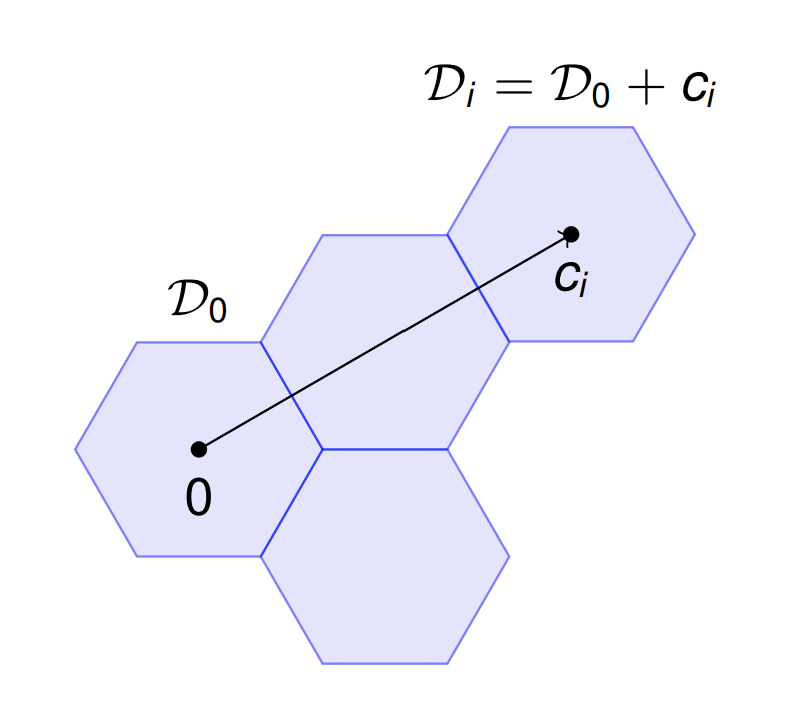
\includegraphics[scale=0.5]{12025-05-20.png}
    \end{center}
    The union of all $\mathcal{D}_i$ is $\mathbb{F}^n$. Hence every $y \in \mathbb{F}^n$ is in exactly one decoding region.
\end{parag}
\begin{parag}{How to implement}
    To find the codeword associated to a channel output $y$, we could find $y$ in the standard array and read out the entry on top of the same column.\\
    Storing the whole standard array is impractical (often impossible for large codes).\\
    The first column describes the geometry of all decoding regions. We should be able to leverage on that.
\end{parag}
\begin{parag}{Claim}
    \begin{theoreme}
    In the standard array, each element of a row has the same syndrome as the coset leader.
    \end{theoreme}
    \begin{subparag}{proof}
        \begin{itemize}
		\item The elements of $\left[t_i\right]$ have the form $t_1 + c$ for some $c \in \mathcal{C}$
		\item The syndrome of such element is:
			\begin{align*} 
				(t_1 + c)H^T =  t_1H^T + cH^T =  t_iH^T
			\end{align*}
			Which is the syndrome of the coset leader $t_i$.
        \end{itemize}
    \end{subparag}
\end{parag}
\begin{parag}{Uniquely identifier}
    \begin{theoreme}
    The syndrome uniquely identies the coset leader
    \end{theoreme}
    \begin{subparag}{Proof}
        Let $t_i$ and $t_j$ be coset leaders\\
	Suppose that $t_iH^T = t_j H^T$, then we know that $\left(t_i - t_j\right)H^T = 0$, then by definition we know that $t_i - t_j = c_k \in \mathcal{C}$\\
	And because $t_i - t_j \in \mathcal{C}$ this implies directly that $t_i \equiv t_j \Mod \mathcal{C} \implies t_i + \mathcal{C} = t_j + \mathcal{C}$ which means they are both in the same coset. Since both are in the same coset and both are coset leaders, $t_i = t_j$.
    \end{subparag}
\end{parag}



\begin{parag}{Theorem}
    \begin{theoreme}
    $\vec{y}_1$ and $\vec{y}_2$ have the \important{same syndrome} if and only if they are in the same coset  
    \end{theoreme}
    The is the theorem \nth{46} with the theorem \nth{47}.
    \begin{subparag}{Proof}
        Because this theorem is the theorem 46 $\iff$ theorem 47 kind of the proof is juste the two proofs together. \\
        In the second condition we say that having the same coset implies the same syndrome.
    \end{subparag}
\end{parag}





